\section{A far wake instability for intermediate $\AR$s}


\begin{figure}
  \centering
  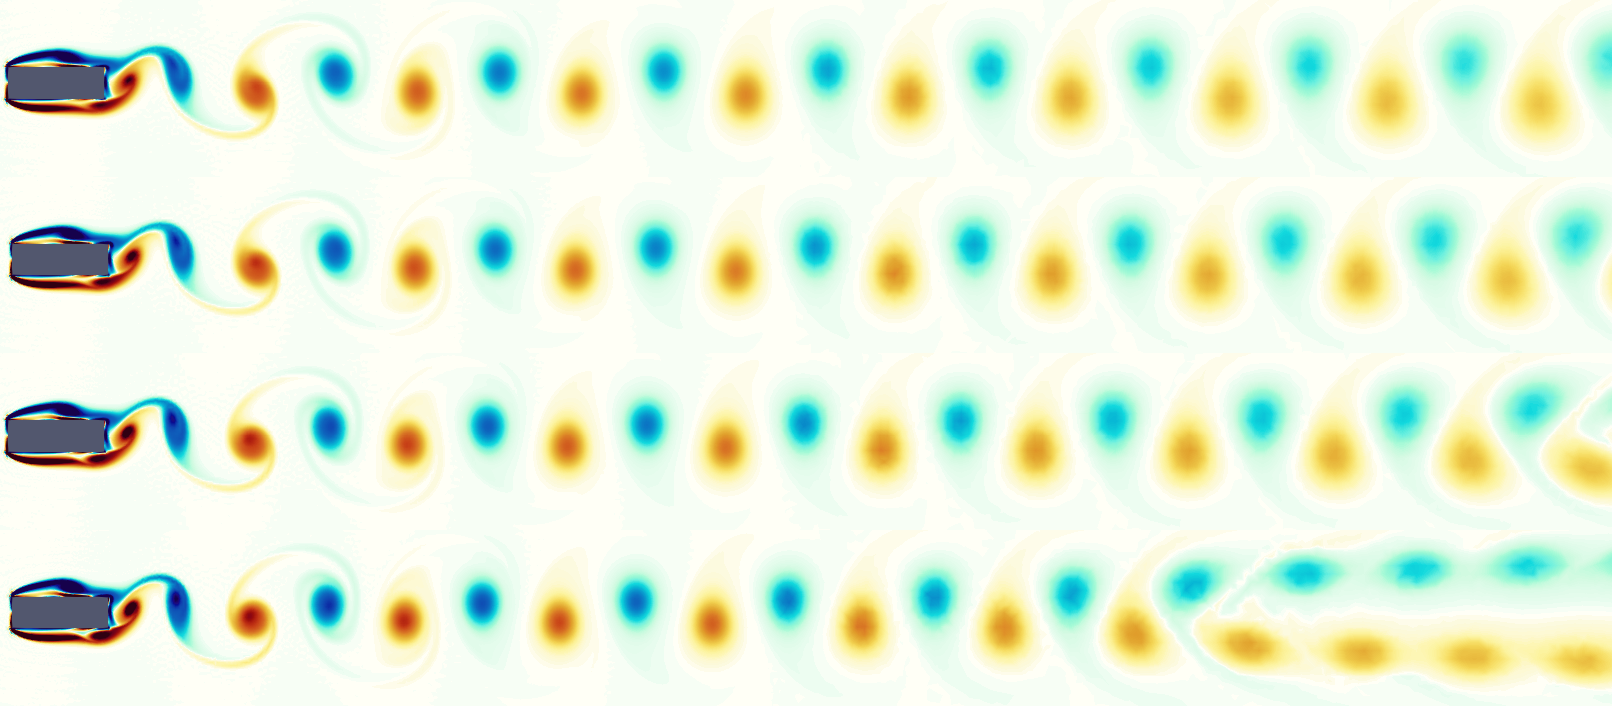
\includegraphics[width=0.8\textwidth]{./fig/AR3/BF_vort_Re400_475.png}
  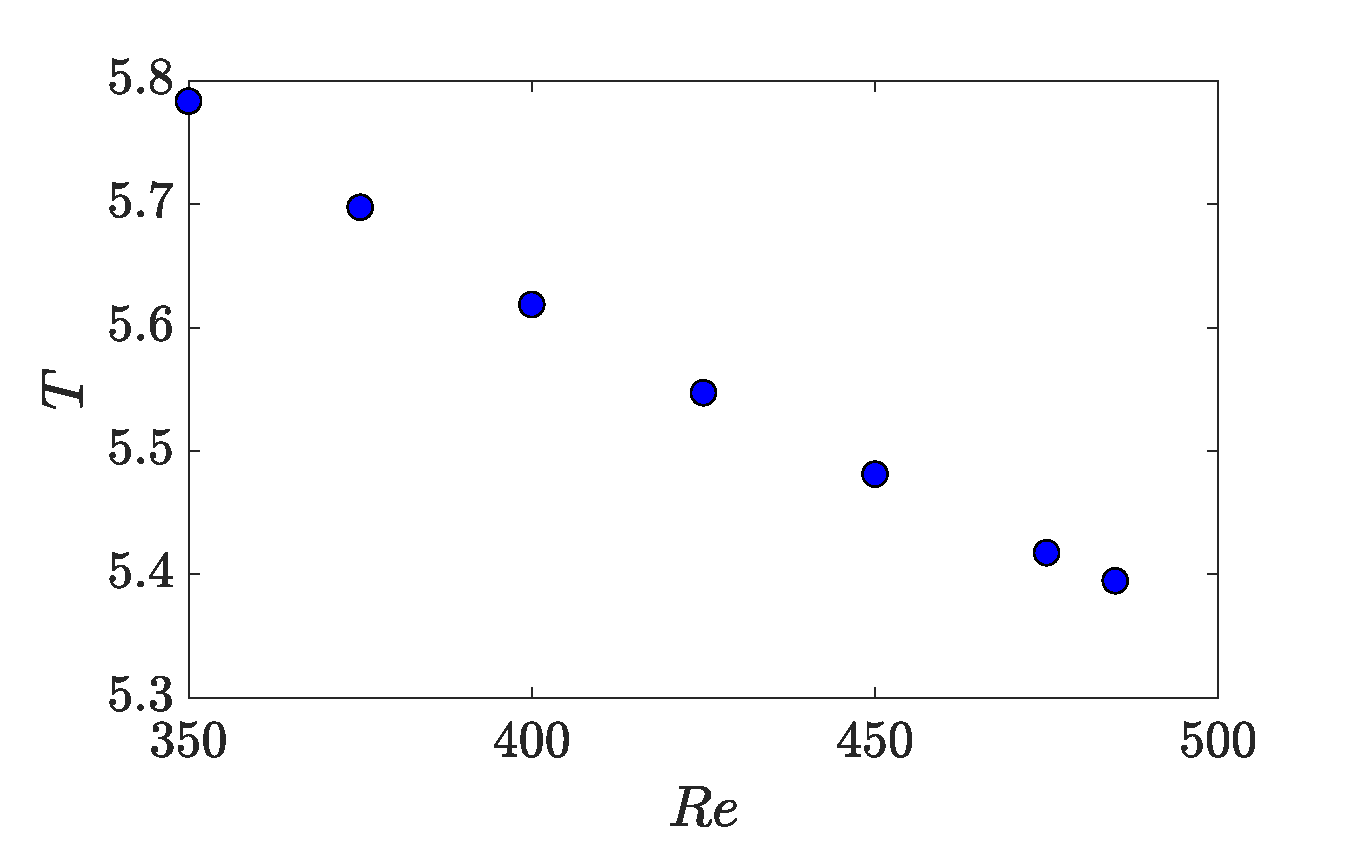
\includegraphics[width=0.5\textwidth]{./fig/AR3/T_Re.eps}
  \caption{Base flow vorticity snapshots for $\AR=3$ at (from top to bottom) $Re=400$, $Re=425$, $Re=450$ and $Re=485$. Note that as $Re$ increases the structure of the wake changes, with the positive and negative vorticity monopoles being clearly separated. As $Re$ increases, this separation start occurring closer to the TE. Bottom panel: Dependence of the period $T$ on $Re$ for the periodic regime in the $350 \le Re \le 485$ range.}
  \label{fig:BF_AR3}
\end{figure}

\begin{figure}
  \centering
  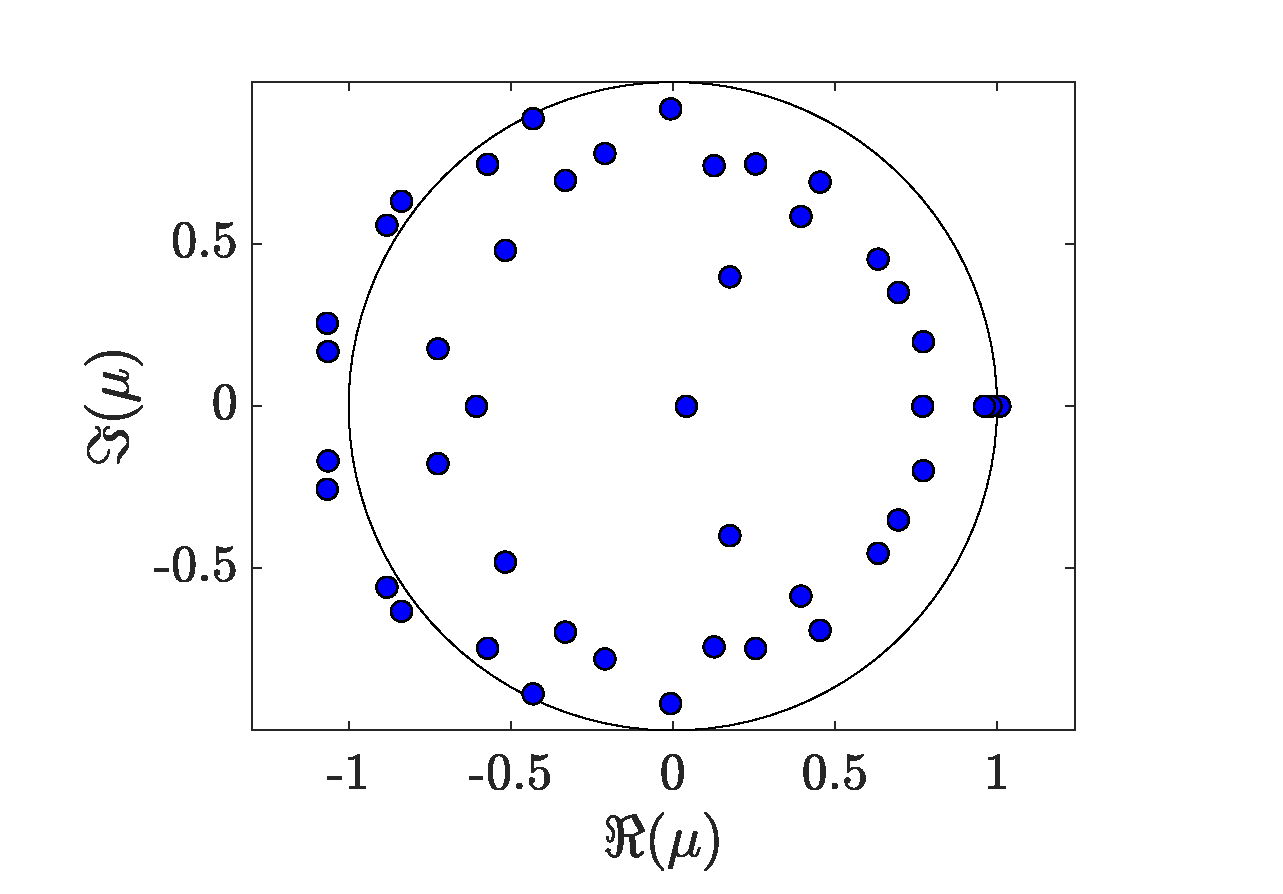
\includegraphics[width=0.5\textwidth]{./fig/AR3/mult_Re495_beta0.eps}
  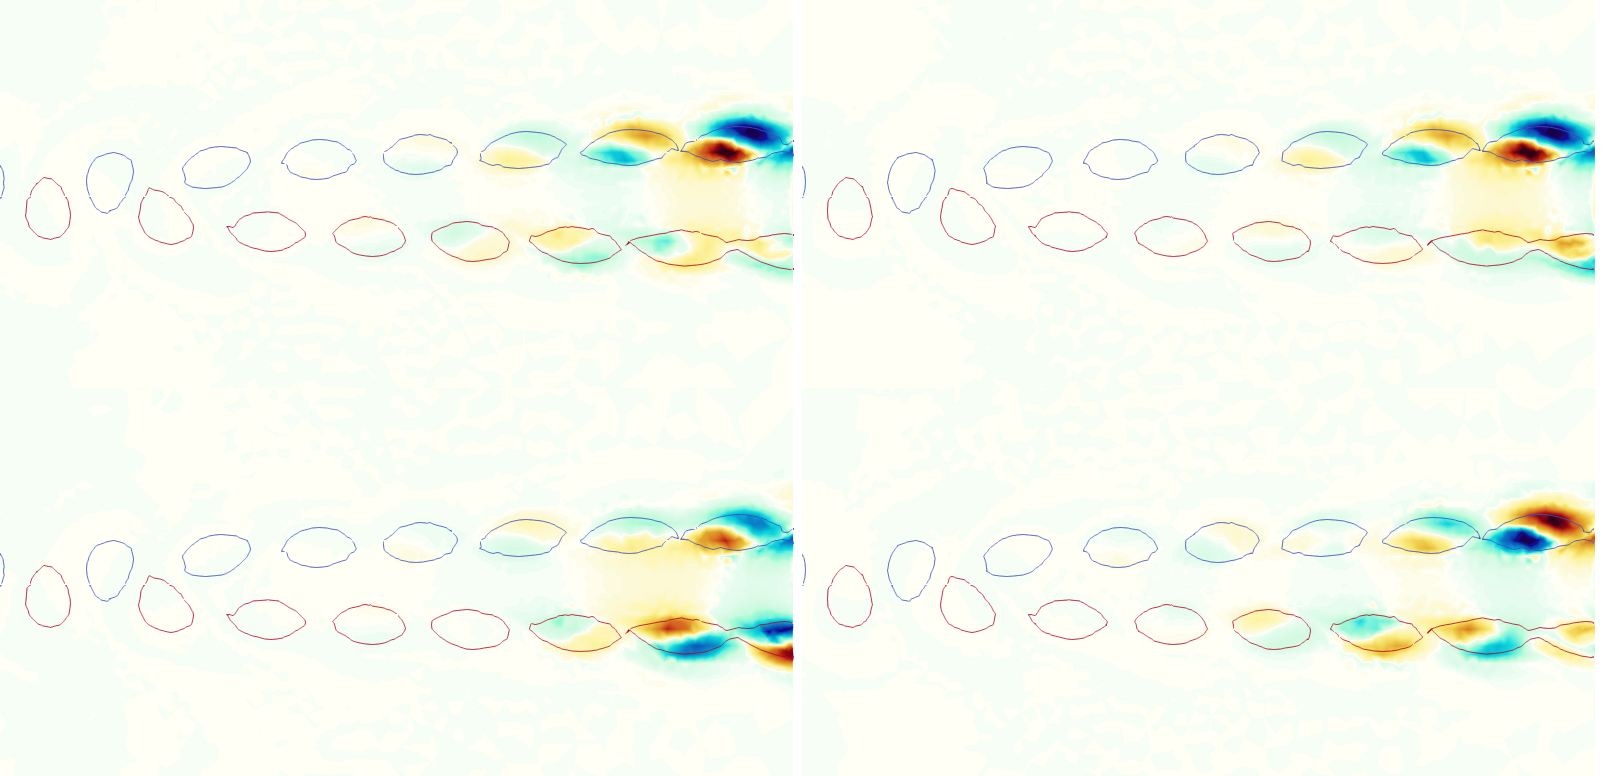
\includegraphics[width=1.0\textwidth]{./fig/AR3/Floquet_modes_beta_0_Re495.png}
  \caption{Floquet analysis for $\AR=3$ and $Re=495$. Top: Floquet multilpiers for $\beta = 0$. Bottom: Modes associated with the $4$ multipliers outside the unit circumference.}
  \label{fig:AR3_Stab}
\end{figure}

\begin{itemize}
  \item For $\AR=3$ we observe that the wake becomes unstable in the far wake.
  \item Study Batchelor and Lamb. Look for instability of trains of vortices
\end{itemize}
